\section{Организационно-экономическая часть}

В данном разделе будет проведен расчет трудоемкости выполнения работ, расчет количества исполнителей,
построение календарного плана, расчет конечной стоимости и экономической эффективности программного продукта (ПП).

\subsection{Введение}

Заказчиком (кафедрой) сформулировано техническое задание на разработку ПП.

Необходимо разработать ПП, осуществляющий распознавание лиц в реальном
времени с приемлемой точностью.

Данный проект выполнен в среде Emacs.
Заказчик предполагает реализовывать ПП на электронном информационном
носителе (компакт-диске).

На рынке подобные продукты представлены как
бесплатными продуктами (OpenCv, PCL), так и коммерческими продуктами (Синезис).

Расчёты производились в соответствии с \cite{econ_1}.

\subsubsection{Организация и планирование процесса разработки}

При использовании традиционного подхода, организация и планирование
процесса разработки программного продукта или программного комплекса
предусматривает выполнение следующих работ:
\begin{itemize}
	\item формирование состава выполняемых работ и группировка их по
	стадиям разработки;
	\item расчет трудоемкости выполнения работ;
	\item установление профессионального состава и расчет количества
	исполнителей;
	\item определение продолжительности выполнения отдельных этапов разработки;
	\item построение календарного графика выполнения разработки;
\end{itemize}

Планирование длительности этапов и содержания проекта осуществляется в
соответствии с ЕСПД ГОСТ 34.603-92 и распределяет работы по этапам,
как показано в таблице~\ref{table:econ_1}.
\begin{table}[ht]
    \centering
	\begin{tabu}[\textwidth]{|c|c|l|}
		\hline
		Основные стадии & № & Содержание работы \\
		\hline
		\multirow{2}{*}{Техническое задание}
			& 1 & Постановка задачи\\
			\cline{2-3}
			& 2 & Выбор средств разработки и реализации\\
		\hline
		\multirow{2}{*}{Эскизный проект}
			& 3 & Разработка математической модели\\
			\cline{2-3}
			& 4 & Разработка алгоритмов расчёта задачи\\
		\hline
		\multirow{3}{*}{Техно-рабочий проект}
			& 5 & Реализация алгоритмов расчёта задачи\\
			\cline{2-3}
			& 6 & Разработка пользовательского интерфейса\\
			\cline{2-3}
			& 7 & Реализация пользовательского интерфейса\\
		\hline
		Внедрение & 8 & Проведение вычислительных экспериментов\\
		\hline
	\end{tabu}
	\captionsetup{justification=centering}
	\caption{Распределение работ по этапам.}
	\label{table:econ_1}
\end{table}

\subsubsection{Расчёт трудоёмкости выполнения работ}

Трудоемкость разработки программной продукции зависит от ряда факторов,
основными из которых являются следующие:
\begin{itemize}
	\item степень новизны разрабатываемого программного комплекса,
	\item сложность алгоритма его функционирования,
	\item объем используемой информации, вид ее представления и способ
	обработки,
	\item уровень используемого алгоритмического языка программирования
\end{itemize}

Исходные данные расчета приведены в таблице~\ref{table:econ_2}
\begin{table}[ht]
    \centering
	\begin{tabu}[\textwidth]{|X[l]|X[l]|}
		\hline
		Функциональное назначение ПП & Управление лицензиями на
		программное обеспечение в техническом университете.\\
		\hline
		Степень новизны разрабатываемого проекта & Группа новизны
		\texttt{B} - разработка программной продукции, имеющей
		аналоги.\\
		\hline
		Степень сложности алгоритма функционирования & \texttt{3}
		группа сложности - программная продукция, реализующая
		алгоритмы стандартных методов решения задач. \\
		\hline
		По виду представления исходной информации & Группа \texttt{12}
		- исходная информация представлена в форме докуметов, имеющих
		одинаковый формат и структуру, требуется форматный контроль
		информации. \\
		\hline
		Структура выходным документов & Группа \texttt{22} - требуется
		вывод на печать одинаковых документов, вывод информационных
		массивов на машинные носители.\\
		\hline
	\end{tabu}
	\captionsetup{justification=centering}
	\caption{Исходные данные}
	\label{table:econ_2}
\end{table}

Трудоемкость разработки программной продукции $\tau_{ПП}$ может быть определена
как сумма величин трудоемкости выполнения отдельных стадий разработки
ПП из выражения:
\begin{equation}
	\tau_{ПП} = \tau_{ТЗ} + \tau_{ЭП} + \tau_{ТП} + \tau_{РП} + \tau_{В}
\label{F:econ_1}
\end{equation}
где
\begin{itemize}
	\item $\tau_{ТЗ}$ - трудоемкость разработки технического задания на
	создание ПП;
	\item $\tau_{ЭП}$ - трудоемкость разработки эскизного проекта ПП;
	\item $\tau_{ТП}$ - трудоемкость разработки технического проекта ПП;
	\item $\tau_{РП}$ - трудоемкость разработки рабочего проекта ПП;
	\item $\tau_{В}$ - трудоемкость внедрения разработанного ПП.
\end{itemize}

Трудоемкость разработки технического задания рассчитывается по формуле:
\begin{equation}
	\tau_{ТЗ} = T_{ЗРЗ} + T_{ЗРП}
\label{F:econ_2}
\end{equation}
где
\begin{itemize}
	\item $T_{ЗРЗ}$ - затраты времени разработчика постановки задач на
		разработку ТЗ, чел. дни;
	\item $T_{ЗРП}$ - затраты времени разработчика программного
		обеспечения на разработку ТЗ, чел. дни.
\end{itemize}

В расчёте участвуют следующие коэффициенты:
\begin{itemize}
	\item $t_{З} = 47$ -- норма времени на разработку ТЗ на программный
		продукт в зависимости от функционального назначения и степени новизны
		разрабатываемого ПП, чел. дни;
	\item $K_{ЗРЗ} = 0,65$ -- коэффициент, учитывающий удельный вес
		трудоемкости работ, выполняемых разработчиком постановки на стадии ТЗ;
	\item $K_{ЗРП} = 0,35$ -- коэффициент, учитывающий удельный вес
		трудоемкости работ, выполняемых разработчиком программного обеспечения
		на стадии ТЗ.
\end{itemize}

Тогда
\begin{equation}
	\tau_{ТЗ} = 47 \cdot (0,65 + 0,35) = 47 [чел. дни]
\label{F:econ_3}
\end{equation}

Аналогично рассчитывается трудоёмкость эскизного проекта ПП $\tau_{ЭП}$:
\begin{equation}
	\tau_{ЭП} = t_{ЭП} \cdot (K_{ЭРЗ} + K_{ЭРП}) = 67 \cdot (0,75 + 0,25) = 67 [чел. дни]
\label{F:econ_4}
\end{equation}

Трудоемкость разработки технического проекта $\tau_{ТП}$ зависит от функционального
назначения ПП, количества разновидностей форм входной и выходной информации
и определяется как сумма времени, затраченного разработчиком постановки
задач и разработчиком программного обеспечения, т.е.
$$\tau_{ТП} = (t_{ТРЗ} + t_{ТРП}) \cdot К_{В} \cdot К_{р}$$
$$К_{В} = (К_{П} n_{П} + К_{НС} n_{НС} + К_{Б} n_{Б} )/(n_{П} + n_{НС} + n_{Б})$$
где
\begin{itemize}
	\item $t_{ТРЗ} = 57, t_{ТРП} = 43$ - норма времени, затрачиваемого на
		разработку технического проекта разработчиком постановки задач и
		разработчиком ПП соответственно, чел.-дни
	\item $K_{p} = 1,26$ - коэффициент учета режима обработки информации
	\item $К_{П} = 1, К_{Н}С = 0,72, К_{Б} = 2, 18$ - значения
		коэффициентов учета вида используемой информации для переменной,
		нормативно-справочной информации и баз данных соответственно
	\item $n_{П} = 6, n_{Н}С = 4, n_{Б} = 0$ - значения коэффициентов
		учета вида используемой информации для переменной,
		нормативно-справочной информации и баз данных соответственно
\end{itemize}

Тогда
$$\tau_{ТП} = (57 + 43)(1 \cdot 6 + 0,72 \cdot 4 + 2,18 \cdot 0)/(6 + 4 + 0)
\cdot 1,26 = 112 [чел. дни]$$

Трудоемкость разработки рабочего проекта $\tau_{РП}$ зависит от функционального
назначения ПП, количества разновидностей форм входной и выходной информации,
сложности алгоритма функционирования, сложности контроля информации,
степени использования готовых программных модулей, уровня алгоритмического
языка программирования и определяется по формуле:
$$\tau_{РП} = К_{к} К_{р} К_{Я} К_{З} К_{ИА} (t_{РРЗ} + t_{РРП})$$
$$K_{ИА} = (К^{'}_{П} \cdot n_{П} + К^{'}_{НС} \cdot n_{НС} + К^{'}_{Б} \cdot
n_{Б})/(n_{П} + n_{НС} + n_{Б} )$$

\begin{itemize}
	\item $t_{РРЗ} = 138, t_{РРП} = 979$ - норма времени, затраченного на
		разработку РП на алгоритмическом языке высокого уровня разработчиком
		постановки задач и разработчиком программного обеспечения соответственно,
		чел.дни.
	\item $K_{K} = 1$ - коэффициент учета сложности контроля информации;
	\item $K_{P} = 1,32$ - коэффициент учета режима обработки информации
	\item $K_{Я} = 1$ - коэффициент учета уровня используемого
		алгоритмического языка программирования;
	\item $K_{З} = 0,8$ - коэффициент учета степени использования готовых
		программных модулей;
	\item $K_{ИА}$ - коэффициент учета вида используемой информации и
		сложности алгоритма ПП;
	\item $К^{'}_{П} = 1,20, К_{Н}С^{'} = 0,65, К^{'}_{Б} = 0,54$ -
		значения коэффициентов учета сложности алгоритма ПП и вида
		используемой информации для переменной, нормативно-справочной
		информации и баз данных соответственно.
\end{itemize}

Тогда
$$К_{ИА} = 6 \cdot 1,20 + 4 \cdot 0,65/(4 + 6) = 0,98$$
$$\tau_{РП} = 1 \cdot 1,32 \cdot 1 \cdot 0,8 \cdot 0,98 \cdot (138 + 979) = 1117 [чел. дни]$$

Так как при разработке ПП стадии «Технический проект» и «Рабочий
проект» объединены в стадию «Техно-рабочий проект», то трудоемкость ее
выполнения $\tau_{ТРП}$ определяется по формуле
$$\tau_{ТРП} = 0,85\tau_{ТП} + \tau_{РП} = 0,85 \cdot 112 + 1117 = 1212 [чел. дни]$$

Трудоемкость выполнения стадии внедрения $\tau_{В}$ может быть рассчитана
по формуле:
$$\tau_{В} = К_{к} К_{р} К_{З} (t_{ВРЗ} + t_{ВРП} ) = 1 \cdot 1,32 \cdot 0,8(33 + 98) = 138 [чел.дни]$$

Трудоемкости по этапам разработки проекта представлены в
таблице~\ref{table:econ_3}.
\begin{table}[ht]
    \centering
	\begin{tabu}[\textwidth]{|X[c]|X[c]|}
		\hline
		Этап & Трудоемкость этапа, [чел. дни]\\
		\hline
		ТЗ & 47\\
		\hline
		ЭП & 67\\
		\hline
		ТРП& 1212\\
		\hline
		В & 138\\
		\hline
		Итого & 1464\\
		\hline
	\end{tabu}
	\captionsetup{justification=centering}
	\caption{Трудоемкости по стадиям разработки проекта}
	\label{table:econ_3}
\end{table}

Средняя численность исполнителей при реализации проекта разработки Q
и внедрения ПО определяется соотношением $N = \frac{Q_{p}}{F}$, где
\begin{itemize}
	\item $Q_{p} = \tau \cdot t_{p}$ - затраты труда на выполнение проекта
		(разработка и внедрение ПО),
	\item $F = T \cdot F_{M}$ - фонд рабочего времени;
	\item $Т$ - время выполнения проекта в месяцах. T = 5 мес.;
	\item $F_{M}$ - фонд времени в текущем месяце, который рассчитывается
		из учета общества числа дней в году, числа выходных и праздничных дней
		и определяется соотношением $F_{M} =
		\frac{t_{p}(D_{k}-D_{B}-D{П}}{12}$
	\item $t_{p}$ - продолжительность рабочего дня;
	\item $D_{K}$ - общее число дней в году;
	\item $D_{B}$ - число выходных дней в году;
	\item $D_{П}$ - число праздничных дней в году.
\end{itemize}

Тогда
$$F = 5 \cdot 8(365 - 103 - 13)/12 = 830$$
$$N = 1464 \cdot 8/830 = 14 - число \quad исполнителей\quad проекта.$$


\subsubsection{Календарный план-график}

Планирование и контроль хода выполнения разработки проводится по
календарному графику выполнения работ. Планирование процесса разработки и
календарный ленточный план представлены в таблице~\ref{table:econ_4}
и рис.~\ref{pic:econ_1} соответственно.

Вывод: при распараллеливании работы ведущего инженера и программи-
стов можно добиться сокращения срока разработки и внедрения программ-
ного продукта с 1464 дней до 211 дней, т. е. в 6,94 раза по сравнению со
временем разработки одним человеком.

В таблице~\ref{table:econ_5} приведены затраты на заработную плату и
отчисления на социальное страхование в пенсионный фонд, фонд
занятости и фонд обязательного медицинского страхования (30\%). Для
всех исполнителей предполагается оклад в размере 20000 рублей в месяц.

Расходы на материалы, необходимые для разработки программной продукции, указаны в таблице~\ref{table:econ_6}.

В работе над проектом используется специальное оборудование – персональные
электронно-вычислительные машины (ПЭВМ) в количестве 14 шт.
Стоимость одной ПЭВМ составляет 20 000 рублей. Согласно нормативным
документам, срок амортизации ПЭВМ составляет 3 года, что определяет
месячную норму амортизации K = 2,7\%.

Тогда за 10 месяцев работы расходы на амортизацию составят $20 000 \cdot 14\cdot
0,027 \cdot 10 = 75 600руб.$

Общие затраты на разработку ПП составят:
$$C = 728 000 + 1 900 + 75 600 = 805 500 руб.$$

\begin{table}
    \centering
	\begin{tabu}[\textwidth]{|X[l]|X[l]|X[c]|X[l]|X[l]|}
	\hline
	Стадия & $\tau$ & Должность исполнителя & Распределение трудоемкости & Ч-ть \\
	\hline
	\multirow{2}{*}{ТЗ} & 47 & Ведущий инженер & 37(79\%) & 1 \\
			& & Программист & 10 & 1 \\
	\hline
	\multirow{2}{*}{ЭП} & 67 & Ведущий инженер & 37(55\%) & 1 \\
			& & Программист & 30 & 1 \\
	\hline
	\multirow{2}{*}{ТРП} & 1212 & Ведущий инженер & 81 & 1 \\
				& & Программист & 13 х 87 & 13 \\
	\hline
	\multirow{2}{*}{B} & 138 & Ведущий инженер & 38 & 1 \\
			 & & Программист & 2 x 50 & 2 \\
	\hline
	Итого & 1464 & & & 14 \\
	\hline
	\end{tabu}
	\captionsetup{justification=centering}
	\caption{Планирование процесса разработки.}
	\label{table:econ_4}
\end{table}

\begin{figure}[ht]
	\centering
	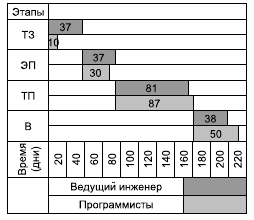
\includegraphics{econ_1.png}
	\caption{Календарный ленточный план работ.}
	\label{pic:econ_1}
\end{figure}

\begin{table}
    \centering
	\begin{tabularx}{\textwidth}{|c||X|X|X||X|X|X||X|X|X||X|X|X||c|}
		\hline
		& \multicolumn{3}{c||}{Г.И.} & \multicolumn{3}{c||}{П1} &
		\multicolumn{3}{c||}{П2} & \multicolumn{3}{c||}{П3..14} & Всего\\
		\hline
		Месяц & Р.Д. & ЗП & ЕСН & Р.Д. & ЗП & ЕСН & Р.Д & ЗП & ЕСН &
		Р.Д. & ЗП & ЕСН & за период\\
		\hline
		1 & 21 & 20 & 6 & 10 & 9.52 & 2.85 & & & & & & & 38.38\\
		\hline
		2 & 21 & 20 & 6 & 5 & 4.76 & 1.42 & & & & & & & 32.19\\
		\hline
		3 & 21 & 20 & 6 & 21 & 20 & 6 & & & & & & & 52\\
		\hline
		4 & 21 & 20 & 6 & 14 & 13.33 & 4 & 7 & 6.66 & 2 & 7 & 6.66 & 2 & 60.67\\
		\hline
		5 & 21 & 20 & 6 & 21 & 20 & 6 & 21 & 20 & 6 & 21 & 20 & 6 & 104.00\\
		\hline
		6 & 21 & 20 & 6 & 21 & 20 & 6 & 21 & 20 & 6 & 21 & 20 & 6 & 104.00\\
		\hline
		7 & 21 & 20 & 6 & 21 & 20 & 6 & 21 & 20 & 6 & 21 & 20 & 6 & 104.00\\
		\hline
		8 & 15 & 14.28 & 4.28 & 21 & 20 & 6 & 21 & 20 & 6 & 14 & 13.33 & 4 & 87.90\\
		\hline
		9 & 21 & 20 & 6 & 21 & 20 & 6 & 21 & 20 & 6 & & & & 78.00\\
		\hline
		10 & 10 & 9.52 & 2.85 & 22 & 20.95 & 6.28 & 22 & 20.95 & 6.28 & & & & 66.86\\
		\hline
		\multicolumn{13}{|l||}{Итого: } & 728.00 \\
		\hline
	\end{tabularx}
	\captionsetup{justification=centering}
	\caption{Затраты на зарплату и отчисления на социальное страхование, тыс.руб.}
	\label{table:econ_5}
\end{table}

\begin{table}[ht]
    \centering
	\begin{tabu}[\textwidth]{|X[c]|X[c]|X[c]|X[c]|X[c]|}
	\hline
	Наименование материала & Единица измерения & К-во & Цена/ед. (руб.) & Сумма (руб.) \\
	\hline
	Персональный компьютер & ASUS K52-JT & 14 & 25000 & 350000 \\
	\hline
	Офисная мебель & стулья и столы ikea & 14 & 5000 & 70000 \\
	\hline
	Бумага А4 & Пачка 500 листов & 2 & 200 & 400 \\
	\hline
	Картридж принтера Canon IP5200 & Картридж, 10мл & 5 & 300 & 1500 \\
	\hline
	\multicolumn{4}{|l|}{Итого:} & 421900 \\
	\hline
	\end{tabu}
	\captionsetup{justification=centering}
	\caption{Затраты на материалы.}
	\label{table:econ_6}
\end{table}

\subsubsection{Расчёт стоимости программного продукта}

Цена ПП рассчитывается по формуле:
$$Ц = С + Пр$$
$$Пр = \frac{(C - C_{M}) \cdot p_{Н}}{100\%}$$
где
\begin{itemize}
	\item $С$ - затраты на разработку ПП
	\item $С{м}$ - материальные затраты, руб./изд
	\item $Пр$ - желаемая прибыль
	\item $р_{н}$ - норматив рентабельности, принимаемый разработчиком
\end{itemize}

Тогда примем $Ц = 5 000 руб.$

Нужно продать 350 лицензионные копии, чтобы окупить вложенные средства.

\subsection{Рассчет экономической эффективности}

Основными показателями экономической эффективности является чистый
дисконтированный доход (ЧДД) и срок окупаемости вложенных средств.

Чистый дисконтированный доход определяется по формуле:
$$ЧДД = \sum^{T}_{t=0}(R_{t} - З_{t}) \frac{1}{(1 + E)^t}$$
где
\begin{itemize}
	\item $T$ - горизонт расчета по месяцам;
	\item $t$ - период расчета;
	\item $R_{t}$ - доход за текущий месяц;
	\item $З_{t}$ затраты за текущий месяц;
	\item $E$ - приемлемая для инвестора норма прибыли на вложенный капитал.
\end{itemize}

Коэффициент E установим равным ставке рефинансирования ЦБ РФ --
8.25\% годовых (или 0, 66\% в месяц). В виду особенности разрабатываемого
продукта он может быть продан лишь однократно. Коэффициент дисконти-
рования равен 1/(1 + Е) = 0,993.

В таблице~\ref{table:econ_6} приведен расчет ЧДД по месяцам работы над проектом.
График ЧДД приведён на рис.~\ref{pic:econ_2}.

\begin{table}
    \centering
	\begin{tabu}[\textwidth]{|c|c|c|c|c|}
	\hline
	Месяц & Тек. Затр. & Общ. Затр. & Тек.доход & ЧДД \\
	\hline
	1 & 46130,95 & 46130,95 & 0,00 & -45817,25 \\
	\hline
	2 & 39940,48 & 86071,43 & 0,00 & -85216,39 \\
	\hline
	3 & 59750,00 & 145821,43 & 0,00 & -143755,76\\
	\hline
	4 & 68416,67 & 214238,10 & 0,00 & -210330,39\\
	\hline
	5 & 111750,00 & 325988,10 & 0,00 & -318332,22\\
	\hline
	6 & 111750,00 & 437738,10 & 0,00 & -425599,63\\
	\hline
	7 & 111750,00 & 549488,10 & 0,00 & -532137,62\\
	\hline
	8 & 95654,76 & 645142,86 & 0,00 & -622710,94\\
	\hline
	9 & 85750,00 & 730892,86 & 0,00 & -703353,54\\
	\hline
	10 & 74607,14 & 805500,00 & 987500,00 & 149328,11 \\
	\hline
	\end{tabu}
	\captionsetup{justification=centering}
	\caption{Расчёт ЧДД (все значения в руб.).}
	\label{table:econ_6}
\end{table}

\begin{figure}
    \centering
	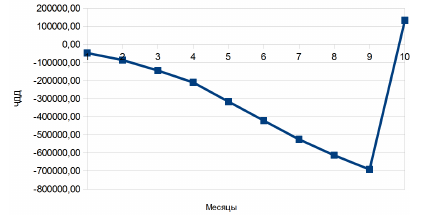
\includegraphics{econ_2.png}
	\caption{График изменения чистого дисконтированного дохода.}
	\label{pic:econ_2}
\end{figure}

\subsection*{Выводы}
\addcontentsline{toc}{subsection}{Выводы}

Согласно проведённым расчётам, проект является рентабельным. Итоговый
ЧДД составил $149328.11$ рублей. Срок реализации проекта равен 10 месяцам.

Поскольку программный продукт - рентабелен, он окупится после выхода на рынок.
Учитывая курс правительства РФ на модернизацию науки и техники, следует
ожидать повышенный спрос не только на конкретную реализацию, а также на
научный труд, подкрепляющий данную реализацию. Также данный программный
продукт может быть использован в широком спектре ниш: распознавание в метро,
при входе на предприятие, автоматическая блокировка ПК, домашние двери.
Это позволяет предположить, что программный продукт не только окупится,
но и принесет ощутимую прибыль при его должном развитии.
\clearpage
